\documentclass[11pt]{article}
%\usepackage{graphicx}
\usepackage{booktabs}
\usepackage[backend=bibtex]{biblatex}
%\addbibresource{myBibRefsFile.bib}
%\usepackage[backend=bibtex,style=verbose-trad2]{biblatex}
\bibliography{IT.bib}
\usepackage{float}

%\usepackage[margin=1in]{geometry}
\usepackage{fancyhdr}
%\pagestyle{fancy}
\usepackage{amsmath}
%\usepackage{amssymb}
%\usepackage[table]{xcolor}
\usepackage{bm}
\usepackage{array}
\usepackage{mathtools}
\usepackage{soul,soulutf8}
\usepackage{url,color}
\usepackage{fullpage}
\usepackage[english]{babel}

\usepackage[utf8]{inputenc}
\lhead{STA 4001: Stochastic Processes}
\chead{}
\rhead{\textup{CUHK(SZ) Fall 2018}}


\usepackage{amsmath,amsthm,amssymb}
%\usepackage{extarrows}
%\usepackage{breqn}
\usepackage{mathtools}
\DeclarePairedDelimiter\ceil{\lceil}{\rceil}
\DeclarePairedDelimiter\floor{\lfloor}{\rfloor}
\newcommand{\N}{\mathbb{N}}
\newcommand{\Z}{\mathbb{Z}}
\newcommand{\trans}{^{\mathrm T}}

\newenvironment{theorem}[2][Theorem]{\begin{trivlist}
\item[\hskip \labelsep {\bfseries #1}\hskip \labelsep {\bfseries #2.}]}{\end{trivlist}}
\newenvironment{lemma}[2][Lemma]{\begin{trivlist}
\item[\hskip \labelsep {\bfseries #1}\hskip \labelsep {\bfseries #2.}]}{\end{trivlist}}
\newenvironment{exercise}[2][Exercise]{\begin{trivlist}
\item[\hskip \labelsep {\bfseries #1}\hskip \labelsep {\bfseries #2.}]}{\end{trivlist}}
\newenvironment{reflection}[2][Reflection]{\begin{trivlist}
\item[\hskip \labelsep {\bfseries #1}\hskip \labelsep {\bfseries #2.}]}{\end{trivlist}}
\newenvironment{proposition}[2][Proposition]{\begin{trivlist}
\item[\hskip \labelsep {\bfseries #1}\hskip \labelsep {\bfseries #2.}]}{\end{trivlist}}
\newenvironment{corollary}[2][Corollary]{\begin{trivlist}
\item[\hskip \labelsep {\bfseries #1}\hskip \labelsep {\bfseries #2.}]}{\end{trivlist}}
\DeclareMathOperator{\tr}{tr}
\DeclareMathOperator{\rank}{rank}
\DeclareMathOperator{\Span}{span}
\DeclareMathOperator{\row}{row}
\DeclareMathOperator{\col}{col}
\DeclareMathOperator{\range}{range}
\DeclareMathOperator{\Null}{Null}
\DeclarePairedDelimiterX{\inp}[2]{\langle}{\rangle}{#1, #2}
\DeclareMathOperator{\Proj}{Proj}
\newcommand{\diff}{\,\mathrm{d}}
\DeclareMathOperator{\trace}{trace}
\newcommand{\Her}{^{\mathrm H}}
\DeclareMathOperator{\diag}{diag}
\newcommand{\Var}{\mathrm{Var}}
%\usepackage{listings}
%\usepackage{color} %red, green, blue, yellow, cyan, magenta, black, white
%\definecolor{mygreen}{RGB}{28,172,0} % color values Red, Green, Blue
%\definecolor{mylilas}{RGB}{170,55,241}
%
%
%\lstset{language=Matlab,%
%    %basicstyle=\color{red},
%    breaklines=true,%
%    morekeywords={matlab2tikz},
%    keywordstyle=\color{blue},%
%    morekeywords=[2]{1}, keywordstyle=[2]{\color{black}},
%    identifierstyle=\color{black},%
%    stringstyle=\color{mylilas},
%    commentstyle=\color{mygreen},%
%    showstringspaces=false,%without this there will be a symbol in the places where there is a space
%    numbers=left,%
%    numberstyle={\tiny \color{black}},% size of the numbers
%    numbersep=9pt, % this defines how far the numbers are from the text
%    emph=[1]{for,end,break},emphstyle=[1]\color{red}, %some words to emphasise
%    %emph=[2]{word1,word2}, emphstyle=[2]{style},    
%}
\usepackage{listings}
\RequirePackage{listings}
\usepackage{graphicx}\usepackage{subfigure}
\RequirePackage{xcolor}
\definecolor{dkgreen}{rgb}{0,0.6,0}
\definecolor{gray}{rgb}{0.5,0.5,0.5}
\definecolor{mauve}{rgb}{0.58,0,0.82}
\lstset{
  frame=tb,
  aboveskip=3mm,
  belowskip=3mm,
  showstringspaces=false,
  columns=flexible,
  framerule=1pt,
  rulecolor=\color{gray!35},
  backgroundcolor=\color{gray!5},
  basicstyle={\small\ttfamily},
  numbers=none,
  numberstyle=\tiny\color{gray},
  keywordstyle=\color{blue},
  commentstyle=\color{dkgreen},
  stringstyle=\color{mauve},
  breaklines=true,
  breakatwhitespace=true,
  tabsize=3,
}

\newcommand{\degree}{\ensuremath{^\circ}}
\begin{document}
\title{\bfseries\upshape{Solution to Assignment 7}}%replace X with the appropriate number
\author{\textit{I will appreciate it if you could give me some advice on my assignment!}} %if necessary, replace with your course title
\maketitle
\begin{enumerate}
\item
The Lagrangian function and its derivatives are given by:
\begin{subequations}
\begin{align}
L(x,\mu)&=\frac{1}{2}\left[-0.1(x_1-4)^2+x_2^2+\mu(1-x_1^2-x_2^2)\right]\\
\nabla_xL(x,\mu)&=\begin{pmatrix}
-0.1(x_1-4)\\x_2
\end{pmatrix}-\mu\begin{pmatrix}
x_1\\x_2
\end{pmatrix}\\
\nabla_{xx}^2L(x,\mu)&=\begin{pmatrix}
-(0.1+\mu)&0\\0&1-\mu
\end{pmatrix}
\end{align}
\end{subequations}
The KKT conditions are given by:
\[
\left\{
\begin{aligned}
\nabla_xL(x,\mu)&=0\\
\mu(1-x_1^2-x_2^2)&=0\\
\mu&\ge0\\
x_1^2+x_2^2&\ge1
\end{aligned}
\right.\Longleftrightarrow
\left\{
\begin{aligned}
x_1&=\frac{4}{1+10\mu}\\
(1-\mu)x_2&=0\\
\mu(1-x_1^2-x_2^2)&=0\\
\mu&\ge0\\
x_1^2+x_2^2&\ge1
\end{aligned}
\right.
\]
\begin{enumerate}
\item
When $\mu=0$, we imply the KKT-point-Lagrangian-multiplier pair
\[
(\bm x*,\mu^*)=(4,0,0).
\]
Since the Hessian at this point is
\[
\bm H=\begin{pmatrix}
-0.1&0\\0&1
\end{pmatrix},
\]
Since $\bm x^*$ is inactive, the active set $V(\bm x^*)$ is the whole space $\mathbb{R}^2$. Also note that this Hessian matrix is \emph{indefinite} on $\mathbb{R}^2$, we imply this KKT point is a saddle point.
\begin{figure}[H]
\centering
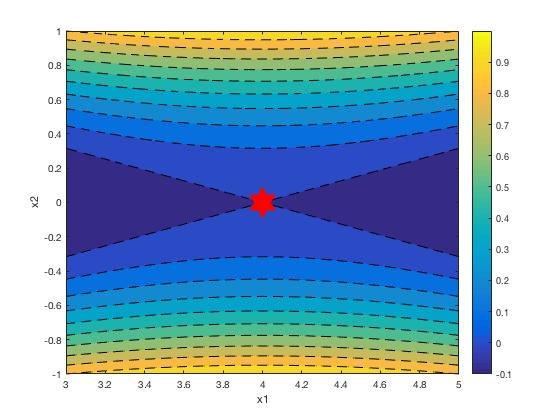
\includegraphics[width=10cm]{A_7_1}
\caption{Contour plot near KKT point $(4,0)$}
\label{Fig:1}
\end{figure}
\paragraph{Interpretation from Fig~(\ref{Fig:1})}We can see that the KKT point $(4,0)$ is strictly inside the constraint, and we can pick a feasible direction that has more/less than $90$ degree angle between the gradient direction, which implies that in some feasible direction $(4,0)$ is local maximum, and in some feasible direction $(4,0)$ is a local minimum. Thus $(4,0)$ is a \emph{saddle point}.
\item
When $\mu=1$, we imply two KKT-point-Lagrangian-multiplier pairs:
\[
(\bm x^*,\mu^*)=\left(\frac{4}{11},\pm\sqrt{1-(\frac{4}{11})^2},1\right)
\]
The Hessian at these two points are negative semi-definite:
\[
\nabla^2_{xx}L(x,1)=\begin{pmatrix}
-1.1&0\\0&0
\end{pmatrix},
\]
and it can be psd only in subspace $\mathcal{O}=\{\bm p\mid\bm p=(0,\alpha),\alpha\in\mathbb{R}\}$. Since in our case it is clear that $V(x^*)\bigcap\mathcal{O}^c\ne\emptyset$, we conclude that these two KKT points cannot be local minimum.
\begin{figure}[H]
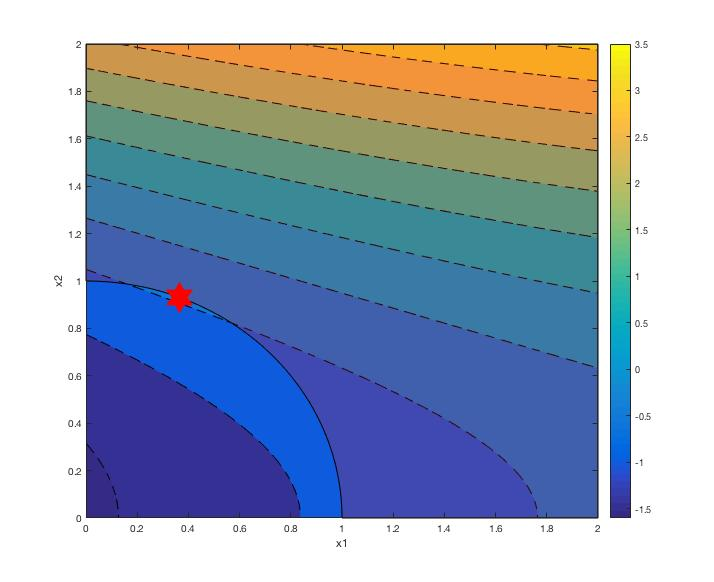
\includegraphics[width=1\textwidth]{A_7_2}
\centering
\caption{Contour plot near KKT point $(4/11,\sqrt{1-(4/11)^2})$}
\label{Fig:2}
\end{figure}
\paragraph{Interpretation from Fig~(\ref{Fig:2})}We can see that the KKT point $(4/11,\sqrt{1-(4/11)^2})$ is on the boundary of the constraint, and we can pick a feasible direction that has more/less than $90$ degree angle between the gradient direction, which implies that in some feasible direction $(4/11,\sqrt{1-(4/11)^2})$ is local maximum, and in some feasible direction $(4/11,\sqrt{1-(4/11)^2})$ is a local minimum. Thus $(4/11,\sqrt{1-(4/11)^2})$ is a \emph{saddle point}.
\begin{figure}[H]
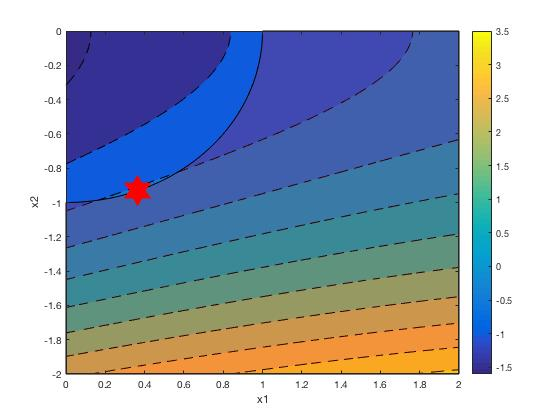
\includegraphics[width=1\textwidth]{A_7_3}
\centering
\caption{Contour plot near KKT point $(4/11,-\sqrt{1-(4/11)^2})$}
\label{Fig:3}
\end{figure}
\paragraph{Interpretation from Fig~(\ref{Fig:3})}We can see that the KKT point $(4/11,-\sqrt{1-(4/11)^2})$ is on the boundary of the constraint, and we can pick a feasible direction that has more/less than $90$ degree angle between the gradient direction, which implies that in some feasible direction $(4/11,-\sqrt{1-(4/11)^2})$ is local maximum, and in some feasible direction $(4/11,-\sqrt{1-(4/11)^2})$ is a local minimum. Thus $(4/11,-\sqrt{1-(4/11)^2})$ is a \emph{saddle point}.
\item
When $\mu\ne1$ and $\mu>0$, we imply the KKT-point-Lagrangian-multiplier pair
\[
(\bm x*,\mu^*)=(1,0,0.3).
\]
The Hessian at this point is given by
\[
\nabla^2_{xx}L(x,1)=\begin{pmatrix}
-0.4&0\\0&0.7
\end{pmatrix}.
\]
The set of points at which $\inp{\nabla h(\bm x^*)}{\bm y}=0$ is given by $V(\bm x^*)=\{\bm y=(0,y_1)\mid y_1\in\mathbb{R}\}$. By Lagrangian multiplier theorem, since $\nabla^2_{xx}L(x,1)$ is positive definite at $V(x^*)$, we imply that this point must be a local minimum.
\begin{figure}[H]
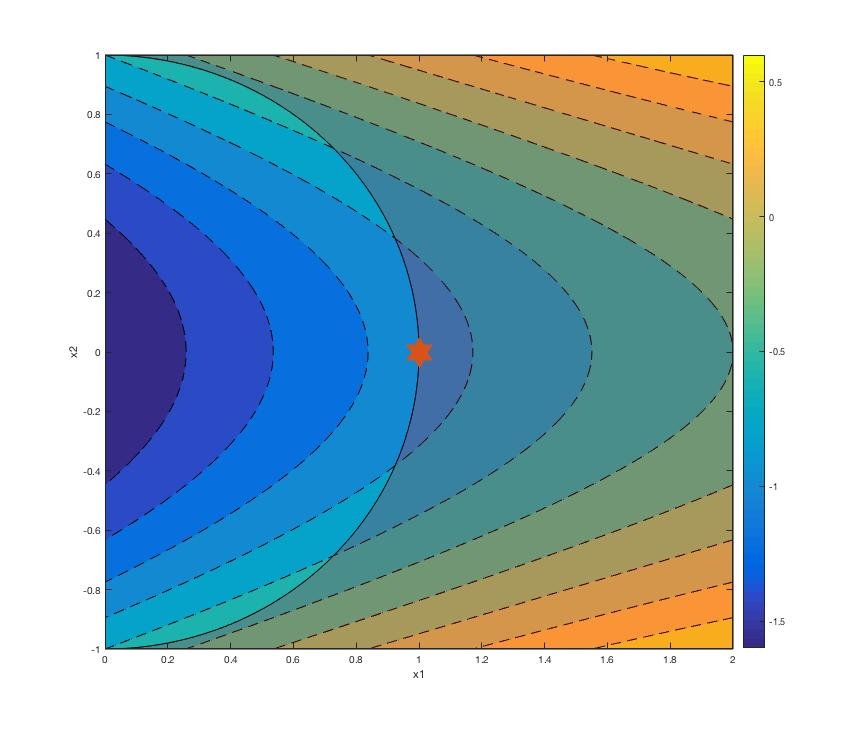
\includegraphics[width=1\textwidth]{A_7_4}
\centering
\caption{Contour plot near KKT point $(1,0)$}
\label{Fig:4}
\end{figure}
\paragraph{Interpretation from Fig~(\ref{Fig:4})}We can see that the KKT point $(1,0)$ is on the boundary of the constraint, and the \emph{gradient} direction at this point is $(1,0)$. From the figure we can also see that the feasible direction at this point should has the \emph{positive $x$-axis component}, which implies that any feasible direction is a ascent direction, i.e., $(1,0)$ is a \emph{local minimum}


\end{enumerate}
In summary, there are four KKT points with multipliers given below:
\[
\begin{array}{ll}
(\bm x_1,\mu_1)=(4,0,0),
&
(\bm x_2,\mu_2)=(\frac{4}{11},\sqrt{1-(\frac{4}{11})^2},1),\\
(\bm x_3,\mu_3)=(\frac{4}{11},-\sqrt{1-(\frac{4}{11})^2},1),
&
(\bm x_4,\mu_4)=(1,0,0.3)
\end{array}
\]
There is only one local minimum point, that is $(\bm x^*,\mu^*)=(1,0,0.3)$.

The code is appendixed in the next page.
\clearpage
\begin{lstlisting}[language=matlab]
%% contour plot
clear
x1 = 4; x2 = 0;
%x1 = 4/11; x2 = sqrt(1-x1^2);
%x1 = 4/11; x2 = -sqrt(1-x1^2);
%x1 = 1; x2 = 0;
x = 3:0.001:5; y = -1:0.001:1;
%x = 0:0.001:2; y = 0:0.001:2;
%x = 0:0.001:2; y = 0:-0.001:-2;
%x = x1-1:0.001:x1+1; y = x2-1:0.001:x2+1;
[X,Y] = meshgrid(x,y);
Z = -0.1 * (X - 4).^2 + Y.^2;
figure
contourf(X,Y,Z,'--');
colorbar;
xlabel('x1')
ylabel('x2')
hold on

n = 1000;
t = linspace(0,pi/2,n);
%t = linspace(0,pi/2,n);
%t = linspace(-pi/2,0,n);
%t = linspace(-pi/2,pi/2,n);
xc1 = cos(t);
yc1 = sin(t);
fill([xc1 0 2 2],[yc1 2 2 0],[1 0 0],'facealpha',0.2)
%fill([xc1 0 2 2],[yc1 2 2 0],[1 0 0],'facealpha',0.2)
%fill([xc1 2 2 0],[yc1 0 -2 -2],[1 0 0],'facealpha',0.2)
%fill([xc1 2 2 0],[yc1 1 -1 -1],[1 0 0],'facealpha',0.2)
scatter(x1,x2,1000,'r','hexagram','field')
%scatter(x1,x2,1000,'r','hexagram','field')
%scatter(x1,x2,1000,'r','hexagram','field')
%scatter(1,0,1000,'hexagram','field')
xlim([3,5]) ylim([-1,1])
%xlim([0,2]) ylim([0,2])
%xlim([0,2]) ylim([-2,0])
%xlim([0,2]) ylim([-1,1])
\end{lstlisting}




\item
The original problem is equivalent to
\begin{equation}\label{Eq:2}
\begin{array}{ll}
-\min&-y\trans x\\
&x\trans Qx\le1
\end{array}
\end{equation}

The Lagrangian function for (\ref{Eq:2}) is given by:
\[
L(x,y,\mu) = -y\trans x+\mu(x\trans Qx-1)
\]

The KKT necessary condition is given by:
\[
\left\{
\begin{aligned}
\nabla L(x,y,\mu)&=0\\
\mu&\ge0\\
\mu(x\trans Qx-1)&=0\\
x\trans Qx&\le1
\end{aligned}
\right.
\Longleftrightarrow
\left\{
\begin{aligned}
-y+2\mu Qx&=0\\
\mu&\ge0\\
\mu(x\trans Qx-1)&=0\\
x\trans Qx&\le1
\end{aligned}
\right.
\]
\begin{enumerate}
\item
When $\mu=0$, we imply from the first condition that the only possibility is $y=0$. Therefore the optimal value is clearly $0$, which can be re-written as $\sqrt{y\trans Q^{-1}y}$.
\item
When $\mu\ne0$, we imply from the first condition that 
\begin{equation}\label{Eq:3}
x=\frac{1}{2\mu}Q^{-1}y.
\end{equation}

Substituting (\ref{Eq:3}) into $x\trans Qx=1$ (by complementarity condition), we derive
\[
\mu^2=\frac{1}{4}y\trans Q^{-1}y\implies
\mu=\frac{1}{2}\sqrt{y\trans Q^{-1}y},
\]
which is strictly positive because of the second condition and the positive definiteness of $Q$. Therefore the optimal solution should be
\[
x=\frac{1}{\sqrt{y\trans Q^{-1}y}}Q^{-1}y,
\]
and therefore the optimal value is given by:
\[
y\trans x=\frac{y\trans Q^{-1}y}{\sqrt{y\trans Q^{-1}y}}=\sqrt{y\trans Q^{-1}y}
\]
\end{enumerate}
To derive the inequality, for the case $x=0$, the inequality is clearly holds since $LHS=0=RHS$. For $x\ne0$, define
\[
s:=\frac{x}{\sqrt{x\trans Qx}}
\]
which follows that $s\trans Qs=\frac{x\trans Qx}{(\sqrt{x\trans Qx})^2}=1$. Thus consider the maximization problem
\begin{equation}\label{Eq:4}
\begin{array}{ll}
\max&y\trans s\\
&s\trans Qs=1
\end{array}
\end{equation}
Note that (\ref{Eq:2}) is a relaxation of problem (\ref{Eq:4}), which implies the optimal value for (\ref{Eq:4}) should be no more than that for (\ref{Eq:2}), i.e.,
\[
\max y\trans s\le \sqrt{y\trans Q^{-1}y}\implies
\frac{y\trans x}{\sqrt{x\trans Qx}}\le \sqrt{y\trans Q^{-1}y}
\]
By rearranging terms we derive:
\[
(y\trans x)^2\le (y\trans Q^{-1}y)\cdot (x\trans Qx)
\]



\end{enumerate}












\end{document}